% Part 2 chapter carrying "Dual-Sector Perturbation Cosmology: A Modified CAMB Implementation with mu < 1, Sigma = 1 and the Sector-Dependent Hubble
% Parameter" (28 Feb 2026), read in full 2026-10-02 (all 595 extracted lines; confirmed in 50-line chunks, ledger complete), in the paper's order. Checks: docs/verification/chains/DUAL_SECTOR_PERTURBATION_CHECK.md.

\chapter{The mechanism in the Boltzmann code: a matter-sector expansion rate}\label{ch:level2}

\section*{Summary}
Chapter~\ref{ch:latetime} tested the dual-sector prediction through MGCAMB's parameterised $\mu$~\cite{Zhao2009MGCAMB,Wang2023MGCAMB}. This chapter puts the mechanism itself into the CAMB~\cite{Lewis2000CAMB}
Fortran source: cold dark matter and baryon perturbations evolve with a matter-sector expansion rate, while photons, neutrinos, recombination and the
background Friedmann equation stay $\Lambda$CDM. The single coupling is $\beta_m=\Omega_m/2=0.15765$ (Planck 2018 $\Omega_m=0.3153$~\cite{Planck2018VI}) with
$E(a)=\exp(1-1/a)$; no parameter is added. Three converged chains against Planck (NPIPE CamSpec TTTEEE~\cite{Rosenberg2022}, low-$\ell$ TT and EE, lensing) give
$\Delta\chi^2=+0.54$ at the best points and $-0.01$ in the chain averages; every standard parameter moves by under $0.1\sigma$; $\sigma_8$ moves from
$0.8087\pm0.0059$ to $0.7998\pm0.0058$ ($-1.1\,\%$). The photon-sector Hubble constant is $67.16\pm0.47$ and the matter-sector value
$67.161\sqrt{1.15765}=72.26$. Two exploratory runs with the term in the background Friedmann equation instead give $H_0\approx61.5$, which Planck excludes.

\section{Why two rates}
The CMB gives $H_0=67.4\pm0.5$ (Planck 2018~\cite{Planck2018VI}); the Cepheid ladder gives $73.04\pm1.04$ (Riess et al.\ 2022~\cite{Riess2022}), with TRGB~\cite{Freedman2021} and lensing time delays~\cite{Wong2020} also
measured locally. Weak lensing has given $S_8$ 2--3$\sigma$ below Planck: KiDS-1000 $0.759^{+0.024}_{-0.021}$~\cite{Asgari2021} (cosmic shear), DES Y3 $0.776\pm0.017$~\cite{DESY3} ($3\times2$pt), HSC Y3 $0.769^{+0.031}_{-0.034}$~\cite{HSCY3} (cosmic shear) \observed;
the completed KiDS survey gives $0.815^{+0.016}_{-0.021}$, in agreement with Planck~\cite{Wright2025}.
Both differences set early-universe photon measurements against late-universe matter measurements. The question here is whether matter and light can
have different effective expansion rates at late times while sharing the early history. Chapter~\ref{ch:latetime} showed that $\mu<1$, $\Sigma=1$ is
consistent with Planck in four data combinations; MGCAMB imposes $\mu$ as a function. Here the mechanism is coded directly.

\observed\ The Planck and Cepheid values differ by $4.9\sigma$, $(73.04-67.4)/\sqrt{0.5^2+1.04^2}$ \calc. The tip of the red giant branch, calibrated with the Hubble and James Webb telescopes and 24 calibrating type Ia supernovae, gives $H_0=70.39\pm1.22\,({\rm stat})\pm1.33\,({\rm sys})\pm0.70\,(\sigma_{\rm SN})$, $\pm1.94$ in quadrature (Freedman et al.\ 2025~\cite{Freedman2025}). It lies $0.97\sigma$ below the matter-sector rate $72.26$ and $1.67\sigma$ above the photon-sector rate $67.16$ \calc: at its present precision the red-giant ladder does not separate the two rates.

\section{Model and implementation}
\subsection{The mechanism}
The background is $\Lambda$CDM,
\begin{equation}
H^2(a)=H_0^2\left[\Omega_ma^{-3}+\Omega_ra^{-4}+\Omega_\Lambda\right],
\end{equation}
and the CDM and baryon perturbations use the matter-sector rate
\begin{equation}
H_m^2(a)=H^2(a)+\beta_mE(a)H_0^2,\qquad E(a)=\exp\!\left(1-\frac1a\right),\qquad\beta_m=\frac{\Omega_m}{2}=0.15765 .
\label{eq:l2_Hm}\end{equation}
The factor $1/2$ is the virial partition (Chapter~\ref{ch:virial}). Photon perturbations use $H(a)$. No field, parameter or change to the action is added.

\subsection{Effective $\mu$ and $\Sigma$}
In the $\mu$--$\Sigma$ language the mechanism is a weaker clustering source for matter with unchanged lensing, $\Sigma=1$. If the modification acted as a
Newton constant scaled by $H^2/H_m^2$,
\begin{equation}
\mu(a)=\frac{H^2(a)}{H^2(a)+\beta_mE(a)H_0^2},\qquad \mu(0)=\frac1{1+\beta_m}=0.864 .
\label{eq:l2_mu}\end{equation}
\begin{center}\small
\begin{tabular}{ccccc}\hline
$z$ & $a$ & $E(a)=e^{-z}$ & $\mu$ (Eq.~\ref{eq:l2_mu}) & $H_m/H$\\\hline
0 & 1.000 & 1.0000 & 0.864 & 1.076\\
0.2 & 0.833 & 0.8187 & 0.905 & 1.051\\
0.5 & 0.667 & 0.6065 & 0.948 & 1.027\\
1 & 0.500 & 0.3679 & 0.982 & 1.009\\
2 & 0.333 & 0.1353 & 0.998 & 1.001\\
3 & 0.250 & 0.0498 & 1.000 & 1.000\\\hline
\end{tabular}
\end{center}
\calc\ How the code realises it. Built with the switch on and off at the Run A parameters, the coded change lowers $\sigma_8$ today by $1.2\,\%$, against
$0.8\,\%$ for Eq.~\eqref{eq:l2_mu} applied as $G_{\rm eff}=\mu G$, with the same redshift dependence (ratios $0.996$ at $z=0.5$, $0.999$ at $z=1$). The coded
mechanism is therefore slightly stronger than Eq.~\eqref{eq:l2_mu}, in the same direction.
The three implementations of the term in the growth equation are compared in Appendix~\ref{app:der:growth}.

\subsection{The CAMB source}
Three changes in CAMB~1.5.8~\cite{Lewis2000CAMB} \texttt{equations.f90}; nothing else is modified.
\begin{enumerate}
\item Module parameters: \verb|iam_beta = 0.15765| and a switch \verb|iam_dual_sector|.
\item The matter-sector rate, after the standard \verb|adotoa| (unchanged):
\begin{Verbatim}[breaklines,breakanywhere,fontsize=\footnotesize]
iam_Ea         = exp(1 - 1/a)
iam_grho0      = grhob + grhoc + grhornomass + grhog + grhov   ! today's total density, 3 H0^2
iam_grho_extra = iam_beta * iam_Ea * a^2 * iam_grho0
adotoa_matter  = sqrt((grho + iam_grho_extra)/3)
\end{Verbatim}
\item The CDM and baryon density equations use it in the metric source:
\begin{Verbatim}[breaklines,breakanywhere,fontsize=\footnotesize]
z_matter = (0.5*dgrho/k + etak)/adotoa_matter    ! standard: /adotoa
clxcdot  = -k*z_matter
clxbdot  = -k*(z_matter + vb)
\end{Verbatim}
\end{enumerate}
The background (\verb|dtauda|), the photon hierarchy, neutrinos, recombination, lensing and the $C_\ell$ calculation are untouched.

\subsection{Parameter count}
\begin{center}\small
\begin{tabularx}{\linewidth}{>{\raggedright\arraybackslash}p{0.16\linewidth}>{\raggedright\arraybackslash}p{0.2\linewidth}>{\raggedright\arraybackslash}X}\hline
Quantity & Status & Origin\\\hline
$\beta_m$ & predicted & virial partition of a $1/r$ potential, applied to all bound structure\\
form of $E(a)$ & from the record constraint & horizon thermodynamics (Chapter~\ref{ch:theory}, Appendix~\ref{app:der:activation})\\
$E(1)=1$ & fixed & definition\\
$\Omega_m$, $H_0$ & standard & Planck 2018\\\hline
\end{tabularx}
\end{center}
The six sampled parameters are those of $\Lambda$CDM: $\{\omega_b,\omega_c,\theta_{\rm MC},\tau,\ln10^{10}A_s,n_s\}$.

\section{Data and method}
Planck: NPIPE (PR4) CamSpec TTTEEE at $\ell\ge30$ (Rosenberg, Gratton and Efstathiou 2022~\cite{Rosenberg2022}), Planck 2018 low-$\ell$ TT and EE~\cite{Planck2018V}, and lensing (CMBMarged~\cite{Planck2018VIII}).
Growth (Run D only): seven $f\sigma_8$ points with diagonal errors --- 6dFGS ($z=0.067$)~\cite{Beutler2012}, SDSS MGS ($0.15$)~\cite{Howlett2015}, BOSS DR12 ($0.38$, $0.51$)~\cite{Alam2017}, eBOSS DR16 LRG
($0.70$), ELG ($0.85$) and quasars ($1.48$)~\cite{Alam2021}. Cobaya~\cite{Torrado2021}, $R-1<0.01$~\cite{Gelman1992}. Run A: IAM, Planck. Run C: $\Lambda$CDM, the same code with the switch off, same
likelihoods. Run D: IAM, Planck + growth. Any A--C difference therefore comes from the modification alone. The high-$\ell$ likelihood differs from
Chapter~\ref{ch:latetime} (plik-lite~\cite{Planck2018V}), so $\chi^2$ values are compared within a level, not across.

\section{Results}
\subsection{Planck: Run A against Run C}

\begin{figure}[htbp]\centering
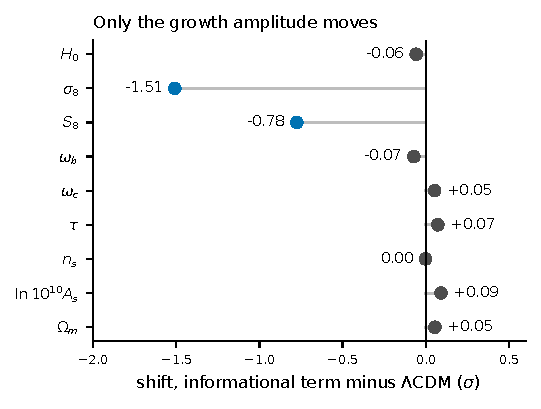
\includegraphics[width=0.6\textwidth]{figures/part2/fig_param_shifts.pdf}
\caption{Shift of each parameter, Run~A (informational term) minus Run~C ($\Lambda$CDM, same code and likelihoods), in units of Run~C's posterior standard deviation, computed from the chain files (\texttt{camb\_validation/\allowbreak{}chains}, 30\,\% burn-in, weighted). Only $\sigma_8$ ($-1.51\sigma$) and $S_8$ ($-0.78\sigma$) move; every other parameter moves by under $0.1\sigma$. \measured}\label{fig:param_shifts}
\end{figure}
\begin{center}\small
\begin{tabular}{lccc}\hline
Parameter & $\Lambda$CDM (C) & IAM (A) & shift\\\hline
$H_0$ & $67.188\pm0.465$ & $67.161\pm0.467$ & $-0.06\sigma$\\
$\sigma_8$ & $0.8087\pm0.0059$ & $0.7998\pm0.0058$ & $-1.51\sigma$\\
$S_8$ & $0.830\pm0.011$ & $0.822\pm0.011$ & $-0.78\sigma$\\
$\omega_b$ & $0.02218\pm0.00013$ & $0.02217\pm0.00013$ & $-0.07\sigma$\\
$\omega_c$ & $0.11989\pm0.00105$ & $0.11994\pm0.00105$ & $+0.05\sigma$\\
$\tau$ & $0.0532\pm0.0073$ & $0.0537\pm0.0073$ & $+0.07\sigma$\\
$n_s$ & $0.9630\pm0.0040$ & $0.9630\pm0.0039$ & $0.00\sigma$\\
$\ln10^{10}A_s$ & $3.0393\pm0.0146$ & $3.0407\pm0.0145$ & $+0.09\sigma$\\
lowest $\chi^2$ & $10972.07$ & $10972.61$ & $\Delta=+0.54$\\
chain-average $\chi^2$ & $10985.08$ & $10985.07$ & $\Delta=-0.01$\\
final $R-1$ & $0.0081$ & $0.0099$ & \\\hline
\end{tabular}
\end{center}
The one parameter that moves is $\sigma_8$, by $-0.009$. $\ln A_s$ ($+0.09\sigma$) and $\omega_c$ ($+0.05\sigma$) barely move, so the shift is not other parameters
compensating: it is slower growth. With the same parameter count, the likelihood ratio is $e^{-0.54/2}=0.76$.

\subsection{Planck + growth: Run D}
Run D does not test the growth rate of the informational term. The coded change acts on the CDM and baryon density equations, while CAMB computes
$f\sigma_8$ from the velocities, which the change does not touch: with the change on, CAMB reports $f=0.542$ at $z=0$ where the density field grows at
$f=0.498$ \measured. Matter is conserved, so the physical growth rate is $f\sigma_8=d\sigma_8/d\ln a$, $6\,\%$ below $\Lambda$CDM today at fixed parameters in
the coded mechanism. A Planck + growth comparison that uses this definition, against a matched $\Lambda$CDM + growth chain, has not yet been run \openprob.
\subsection{The fixed coupling against the chain's $\Omega_m$}
$\beta_m$ is fixed at $0.15765$. In Run A, Planck gives $\Omega_m=0.3166\pm0.0065$, so $\Omega_m/2=0.1583\pm0.0033$: the fixed value is $0.2\sigma$ from it.

\section{The sector-dependent Hubble parameter}

\begin{figure}[htbp]\centering
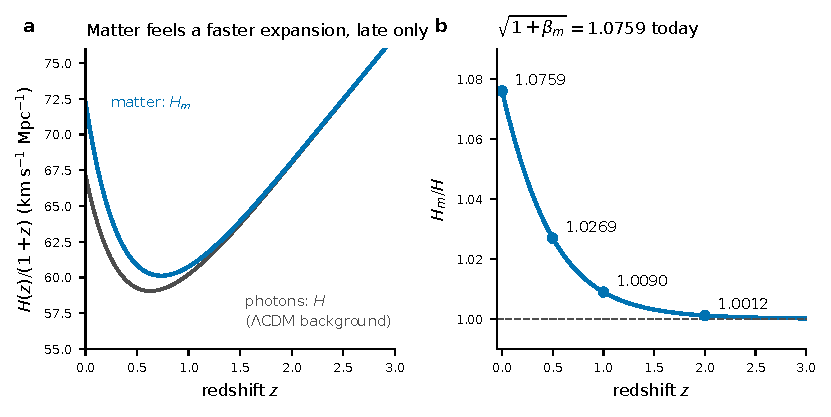
\includegraphics[width=\textwidth]{figures/part2/fig_sector_rates.pdf}
\caption{(a) $H(z)/(1+z)$ for photons (the $\Lambda$CDM background) and for matter, $H_m^2=H^2+\beta_mE(a)H_0^2$, at the Run~A posterior ($H_0=67.161$, $\Omega_m=0.3166$). (b) $H_m/H$: 1.0759 today, 1.0269, 1.0090 and 1.0012 at $z=0.5$, 1 and 2. \calc}\label{fig:sector_rates}
\end{figure}
From Eq.~\eqref{eq:l2_Hm},
\begin{equation}
\frac{H_m(a)}{H(a)}=\sqrt{1+\frac{\beta_mE(a)H_0^2}{H^2(a)}},\qquad\frac{H_m(0)}{H(0)}=\sqrt{1.15765}=1.0759 .
\end{equation}
Run A gives $H_0=67.161\pm0.467$ for the background, the photon sector. The matter-sector value is $H_0^{(m)}=67.161\times1.0759=72.26\pm0.50$.
Against observation: photon $(67.16-67.36)/0.54=-0.37\sigma$ from Planck; matter $(72.26-73.04)/1.04=-0.75\sigma$ from SH0ES.
\begin{center}\small
\begin{tabular}{ccccc}\hline
$z$ & $H$ (photon) & $H_m$ (matter) & ratio & $E(a)$\\\hline
0 & 67.16 & 72.26 & 1.0759 & 1.0000\\
0.5 & 88.89 & 91.29 & 1.0269 & 0.6065\\
1 & 120.44 & 121.53 & 1.0090 & 0.3679\\
2 & 204.06 & 204.29 & 1.0012 & 0.1353\\
3 & 307.37 & 307.43 & 1.0002 & 0.0498\\\hline
\end{tabular}
\end{center}
At $z=2$ the matter-sector rate is $0.1\,\%$ higher; at $z=3$, $0.02\,\%$. The split is a late-time effect, leaving recombination and BBN untouched.

\section{The background test}
Two exploratory chains put $\beta_mE(a)$ into CAMB's background Friedmann equation (\verb|dtauda|) instead. They return $H_0=61.45\pm0.42$ and
$61.52\pm0.43$, $10.9\sigma$ from Planck: the CMB can absorb a background change only by moving $H_0$. The coupling therefore enters through the
perturbations; light travels on the $\Lambda$CDM background.

\section{Discussion}
\subsection{Results}
\begin{center}\small
\begin{tabularx}{\linewidth}{>{\raggedright\arraybackslash}Xcc}\hline
& IAM & $\Lambda$CDM\\\hline
$\sigma_8$ & $0.800\pm0.006$ & $0.809\pm0.006$\\
$S_8$ & $0.822\pm0.011$ & $0.830\pm0.011$\\
$H_0$ (photon) & $67.16\pm0.47$ & $67.19\pm0.47$\\
$H_0$ (matter) & $72.26$ & --\\
$\Delta\chi^2$ Planck (lowest; chain average) & $+0.54$; $-0.01$ & --\\
parameters beyond $\Lambda$CDM & 0 & --\\\hline
\end{tabularx}
\end{center}
\subsection{What this shows, and what it does not}
The coded mechanism, with no new parameter, is indistinguishable from $\Lambda$CDM under Planck, lowers $\sigma_8$ by $1.1\,\%$ toward the weak-lensing
values without degrading any CMB observable, and gives a photon $H_0$ consistent with Planck together with a matter $H_0$ consistent with SH0ES. It does not
show that the Hubble tension is resolved: Planck cannot tell the two models apart. The decisive test is the growth rate at the predicted amplitude.
\subsection{Relation to Chapter~\ref{ch:latetime}}
Both levels lower $\sigma_8$ to $0.800$--$0.802$ from the same $\beta_m$: by $1.6\,\%$ with MGCAMB's $\mu$ (from $0.814$, plik-lite) and $1.1\,\%$ here (from
$0.809$, NPIPE CamSpec).
\subsection{Predictions}
\begin{enumerate}
\item $\mu(z)<1$ with redshift dependence fixed by $E(a)$; Euclid's published forecasts bracket the test of the IAM $\mu(z)$ from about $0.3\sigma$ (conservative scale cuts) to about $7\sigma$ (smallest
scales modelled), and a forecast made with the IAM $\mu(z)$ itself is still to be done (Chapter~\ref{ch:latetime}).
\item $\Sigma=1$ at all redshifts.
\item $H_0^{(m)}/H_0^{(\gamma)}=\sqrt{1+\Omega_m/2}$, testable with standard sirens, whose hosts are galaxies.
\item No scale dependence: $\mu$ and $\Sigma$ depend on $z$ only.
\end{enumerate}

\section{Conclusions}
Three changes to the CAMB source, no new parameter: under Planck, $\Delta\chi^2=+0.54$; $\sigma_8$ $0.809\to0.800$; standard parameters within $0.1\sigma$;
$H_0$ $67.16$ for light and $72.26$ for matter; the background version excluded. All chains, configuration files, the modified source and the scripts are in
\texttt{camb\_validation/\allowbreak{}}.
